\documentclass[11pt]{article}

\usepackage{mathtools} 
\usepackage[utf8]{inputenc}
\usepackage[czech]{babel}
\usepackage[]{algorithm2e}
\usepackage{url}
\usepackage{xcolor}
\usepackage[round, sort]{natbib}
\usepackage{url}

\urlstyle{same}
\bibliographystyle{apalike}

\addto\captionsczech{
  \renewcommand{\contentsname}{Table of contents}%
  \renewcommand{\figurename}{Figure}%
}
\title{Handling Missing Values in Decision Forests in the Encrypted Network Traffic}
\date{2018-05-06}
\author{Lukáš Sahula}

\begin{document}
  \maketitle
  \newpage
  \section*{Acknowledgement}
    {\color{red}TODO}
  \newpage
  \section*{Abstract}
    {\color{red}TODO}
    \\~\\
    {\bf Keywords:} malware, classification, random forests, supervised learning, missing values, imputation 
    \\~\\
    {\color{red}TODO}
    \\~\\
    {\bf Klíčová slova:} malware, klasifikace, náhodné lesy, učení s učitelem, chybějící hodnoty, imputace 
  \newpage
  \tableofcontents
  \newpage

  \section*{Introduction}
  \addcontentsline{toc}{section}{Introduction}
    Machine learning and cybersecurity are two highly significant buzzwords of today's tech industry. With machine learning being considered as the modern cure-all pill it is no wonder that it has found its uses even in the field of cybersecurity. This thesis touches both of these subjects in the context of automated {\it malware classification}, with the main focus being dealing with {\it missing values} using {\it random forests}.
    \\~\\
    In order for any classification algorithm to work, it has to be trained on a sufficient dataset. In this case the datasets are encrypted network proxy logs and as such they contain a moderate amount of {\it missing data}. Most classification algorithms are not designed with an implicit way of dealing with missing values and thus they have to be handled before the classification process.
    \\~\\
    Over the past two decades, a significant number of methods for dealing with missing data has been introduced, but none has yet shown any game-breaking results. Plenty of methods are somewhat situational and work only with specific cases of missing data. Thus it is not clear which method to choose at which time. This thesis studies these methods along with analysing the network proxy log datasets in order to find out the most efficient one.
    \\~\\
    The thesis consists of several sections. At the beginning, there is a brief introduction to malware classification, followed by an explanation of the classification algorithm often connected to the missing data problem - the {\it random forest classifier}. The next chapter concerns itself with missing data mechanisms and gives a summary of known algorithms for missing data {\it imputation}. The chapter after that provides an analysis of the network datasets. The last section is dedicated to the conducted experiments and results of this thesis.
  \newpage
  \section{Malware and classification}
      This chapter serves both as a general introduction to the term {\it malware} and as an introduction to {\it machine learning}, specifically to one of its subsets, {\it classification}. After explaining both terms, there is a short section dedicated to connecting the two terms.
    \subsection{Malware}
      {\it Malware} is an abbreviated form of the term malicious software. It is often used when referring to viruses, spyware, and other software designed to cause harm to a computer, server, network or a mobile device. \citep{malware}
      \\~\\
      Viruses are computer programs with the goal of spreading from one file to another across one or multiple devices through a network undetected and without consent of the user. A common misinterpretation of viruses is that they are programs designed to delete or move data, however, this damage is often a side effect. The definition of a virus is that it spreads itself. \citep{malware}
      \\~\\
      Spyware is a form of computer program that runs on the infected computer and tracks its user's habits to form a pattern that can be then used for advertisements or sent to the spyware's creator. \citep{malware}
      \\~\\
      When malware spreads through the network, or when it communicates with their command and control computers, it leaves a detectable trace in the network traffic. What more, these traces can often be found much sooner (ranging from weeks to months) than security administrators are able to capture a sample of the invading malware. \citep{network} According to the five years long study by Georgia Institute of Technology, the endpoints with which specific malware communicates do not change in long time periods (years). This means that once a node in the network suspicious of being infected is found, it is possible to look for traffic going in and out, which in turn can help with identifying other infected devices. \citep{network}
      \newpage
    \subsection{Classification}
      In statistics and machine learning, classification is the process of assigning a specific category, or a {\it class}, to which a new object or an observation belongs. This assignment, or {\it prediction}, is done after processing a set of previously categorized data, often called the {\it training dataset}. This is done by a classification algorithm, known as a {\it classifier}. This classifier learns from a set of data, for example emails labeled as spam or non-spam, in order to predict the category of new incoming emails. That way an email client can move unwanted spam to the spam folder and keep the relevant mail in the inbox. Another is predicting whether a patient's tumor is benign or malign, based on the hospital records with data from other patients. Or, as will be the case in this thesis, whether an instance of network traffic is the result of (and which) malware, based on data gained from network proxy logs.
      \\~\\
      Within the terminology of machine learning, classification is in the category of {\it supervised learning}. \citep{mlintro} Supervised learning means that the classifier learns from the training dataset with labeled data. This dataset is often in the form of a matrix. The rows in this matrix are called {\it feature vectors}. They contain the observed attributes, called {\it features}, of each individual object. These features are quantifiable and can be categorical (smoker or non-smoker), integer-valued (age of the patient in years), or real-valued (patient's body temperature). Since the learning is supervised, the dataset also includes a column with the class labels of each observed object.
      \\~\\
      When the classifier is trained, it can predict the classes of new objects based on their features. The mathematical function implemented by the classifier maps input feature vectors {\bf x} of a matrix {\bf X} to a class {\bf c}. The performance of the classifier is usually tested on another set of data called the {\it testing dataset}.
      \\~\\
      Classification does not always have to be binary, meaning the data can be of more than two categories. This is called {\it multiclass classification}. Returning to the example of e-mail classification, some classifiers could be trained to predict whether an incoming e-mail belongs to {\it work}, {\it school}, or {\it personal} categories.
      \\~\\
      There are also other forms of classification, like the {\it multilabel classification}. In multilabel classification, multiple classes can be assigned to an observation. This makes sense in cases where the categories are not mutually exclusive. However, this thesis will be focusing only on the problem of multiclass classification.
    \subsection{Malware classification}
      {\color{red}TODO}
  \newpage
  \section{Random forest classifier}
    {\it Random forests} or {\it random forest classifiers} are the central focus of this thesis because they are most suited for the malware classification problem. They can handle {\it multiclass classification}, evaluate data relatively fast and they are not heavily affected by {\it imbalanced datasets}. \citep{brabec} They run efficiently on large amounts of data and give estimates of what feature variables are important for classification. \citep{breiman}
    \\~\\
    This chapter explains in detail how random forests work and how they can be implemented. As the name implies, random forest is an ensemble of learning algorithms called {\it decision trees}. In order to understand random forests, decision trees are the first thing that needs to be explained.
    \subsection{Decision trees}
      \subsubsection{Overview}
        {\it Decision tree classifier} is a classification algorithm probably named because of its structure resembling a decision tree known from graph theory. Another variation of a decision tree is the regression tree, which only differs in that the predicted outcome is not a class but a real value. One of the most significant publications about decision trees is {\it Classification and Regression Trees} by L. Breiman. It introduces the {\it CART algorithm} for growing both classification and regression trees. \citep{cart} Other algorithms for growing decision trees also exist, for example the {\it ID3 algorithm} or the {\it C4.5 algorithm}.
        \\~\\
        A grown tree consists of a root node, decision nodes and terminal nodes, also called {\it leaves}. All leaves are associated with the resulting prediction class. Each decision node contains information about its split, which consists of an attribute, or a {\it feature}, and its value. When an observed object is analysed to predict its class, the value of the feature in question is compared with the value stored at the decision node. Depending on the result of this comparison, the object is then sent to the left child or the right child of the node. When the object reaches a leaf node, it is given the class that is associated with it. This explanation is visualised in Figure \ref{figure:decision_tree}.
        \begin{figure}
          \centering
          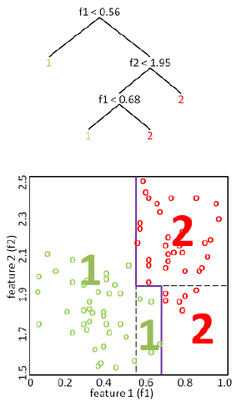
\includegraphics{thesis_res/decision_tree.png}
          \caption{Picture of a decision tree with the training data used for its growth. \citep{digstaining}}
          \label{figure:decision_tree}
        \end{figure}
      \subsubsection{Strengths}
        In comparison with other classification algorithms, decision trees have various strengths and advantages, like:
        \begin{itemize}
        \item They are easily interpretable by people after a brief explanation. The graphical representation of the tree is also very easy to follow and the decision making process is similar to how people generally make decisions in real life. \citep{isl}
        \item They require little data preparation, for example data normalisation is not needed like in other techniques. \citep{isl}
        \item They work with both numerical and categorical data. \citep{isl}
        \item They perform well with large datasets within reasonable time. \citep{breiman}
        \end{itemize}
      \subsubsection{Weaknesses}
        However, decision trees are not perfect as classifiers go because they also have some weaknesses, for example:
        \begin{itemize}
        \item They are not as accurate as other approaches. \citep{isl}
        \item They are not very robust, a small change in training data can lead to a big change in the decision tree, leading to different results. \citep{isl}
        \item They are prone to {\it overfitting}. \citep{isl}
        \end{itemize}
        All these disadvantages are going to be addresed again in the random forests part of this chapter.
    \newpage 
    \subsection{Random forests}
  \newpage
  \section{Handling missing values}
    In statistics, {\it missing values} or {\it missing data} mark the absence of value in a feature variable of an observed sample. Missing data within a dataset make it impossible for conventional machine learning algorithms to properly learn from it. Many of these algorithms require complete data and do not have an implicit way of handling missing values. In order for the statistical analysis to work, the missing data have to be somehow dealt with beforehand. \citep{otfi}
    \\~\\
    There are various ways of handling missing data, some as simple as dropping the samples containing any missing values altogether, leaving only those samples with all data present. \citep{lwd} This however, cannot be done when there are missing data somewhere in most of the observations. Another simple method, the strawman imputation \citep{otfi} would be replacing missing data with the mean or median of all the non-missing values of the feature in question. The process of replacing the missing data is called {\it imputation}.
    \\~\\
    More sophisticated methods of imputation also exist and they are discussed more thoroughly in this thesis. Some methods work better with smaller datasets, or with datasets with low missingness ratio. The amount of correlation between feature variables can also be important to some methods and not that important to others. \citep{otfi} Some imputation algorithms are very slow and using them in experiments with big datasets can get seriously time-consuming. In other words, choosing a relevant method of imputation for a given dataset is not a simple task and it can prove useful to do an analysis of the data as well as an analysis of the imputation algorithm itself beforehand.
    \subsection{Related work}
      Various works comparing different imputation methods were published in the last years. Three imputation methods meant for decision trees are well explained in a paper called {\it Good methods for coping with missing data in decision trees}. \citep{mia}
      \\~\\
      Another work worth mentioning that focuses on random forests and missing data imputation is {\it Random survival forests}. \citep{rsf}
      \\~\\
      Perhaps the most recent work on this topic is {\it Random Forest Missing Data Algorithms} \citep{otfi} which is a continuation of the previous one by one of the same authors. In this paper, five ways of imputation using random forests are discussed in detail and tested on multiple datasets with different attributes. A comparison of their imputation accuracy is made as well.
    \\~\\
    \subsection{Missing data mechanisms}
      Missing data are usually divided into three categories, depending on the characteristics of their missingness. These categories are also called missing data mechanisms. \citep{lwd} It is important to understand these mechanisms in order to make an educated assumption about the dataset in question. If an assumption is made that the values are missing completely at random while they are missing systematically, an analysis based on this assumption may be biased.
      \begin{itemize}
      \item If the samples with missing data are a random subset of all observed samples, they have a similar distribution. There is no relationship between whether a value is missing and any other value in the data set, be it missing or observed. These values are {\it missing completely at random} (MCAR). \citep{lwd} When a dataset has missing values that are MCAR, it can still be analysed with unbiased results, provided that there are enough observed samples. However, data that are truly MCAR are not encountered often.
      \item When the missing data is somehow dependent or related to other non-missing values in the observation, the data is {\it missing at random} (MAR). \citep{lwd} There is no definitive way of distinguishing between MCAR and MAR data. The assumption of it being one or the other is only as good as the knowledge of the data and the field of the one proposing the assumption. A good example of MAR data would be that males are less likely to fill a depression survey, although it does not have any connection to their level of depression.
      \item The last missing data mechanism is {\it missing not at random} (MNAR). It means that there is a relationship between value of the variable that is missing and the reason why it is missing in the first place. For example a male suffering from a strong depression can decide not to fill a depression survey because of said depression.
      \end{itemize}
    \subsection{Selected imputation algorithms}
      This section contains a list of imputation algorithms that were taken in consideration when deciding which ones to implement.
      \begin{itemize}
      \item Strawman imputation
      \item Proximity imputation
      \item On-the-fly-imputation
      \item Missingness incorporated in attributes
      \item Unsupervised imputation
      \item missForest
      \item Surrogate splits
      \end{itemize}
      \subsubsection{On-the-fly-imputation}
        {\it Adaptive tree imputation} \citep{rsf} or {\it On-the-fly-imputation} \citep{otfi} (OTFI) is a method of imputing missing data at the time of growing the tree. It draws a random value from the non-missing in-bag dataset within the current node to impute the missing values. The algorithm works as follows: 
        \begin{enumerate}
        \item First, the best split is calculated as usual, using only non-missing data.
        \item After finding the best split, random values from the non-missing in-bag data within the current node are used to impute the missing values.
        \item Once the data are imputed, the node is split into the left and right children nodes and the imputed data are reset back to missing.
        \end{enumerate}
        The values the algorithm uses to impute the missing data are stored within the decision node while growing the tree along with the respective frequencies in which they occur within the node's dataset. These are then used again to impute the missing values in the testing dataset at the time of prediction to decide whether the observation belongs to the left or to the right child. After being sent to the child node, the imputed data is reset to missing again and the process repeats.
      \subsubsection{Missingness incorporated in attributes}
        {\it Missingness incorporated in attributes} \citep{mia} (MIA) works similarly to OTFI in that it also imputes missing data during the forest growing process. It searches for the best split in three different approaches to the missing data. Let {\it X} be a numeric feature used to split a node and {\it s} a possible split value of {\it X}. Over all split values, the method looks at the following:
        \begin{itemize}
        \item Split A: \{ $X \leq s$ or $X =$ missing \} versus \{ $X > s$ \}.
        \item Split B: \{ $X \leq s$ \} versus \{ $X > s$ or $X =$ missing \}.
        \item Split C: \{ $X =$ missing \} versus \{ $X =$ not missing \}.
        \end{itemize}
        After finding the best split in each approach separately, the algorithm then chooses which one of them provides a better information gain and then it splits the dataset accordingly. As in the OTFI method, the decision node here remembers which split type it had assigned in order to decide how the testing data should be propagated during prediction.
      \subsubsection{Strawman imputation}
        {\it Strawman imputation} \citep{otfi} is a simple method for handling missing values. It works very fast compared to other methods and its implementation is very simple. The missing values are imputed before the forest is grown by calculating the median of non-missing values in the feature column.
        \\~\\
        Considering the implementation is a matter of seconds, an altered version of strawman imputation was also used, one that uses mean instead of median.
        \\~\\
        Further alteration inspired by the on-the-fly-imputation method could be done to strawman imputation. That is, the mean or median could be calculated later during the process of growing a decision tree, at the moment of splitting. But instead of choosing randomly from the in-bag frequencies of non-missing values, mean or median of the in-bag data would be stored at the node and used later for predictions.
  \section{Network dataset}
    {\color{red}TODO}
    \subsection{Dataset description}
      {\color{red}TODO}
    \subsection{Analysis with correlation}
      {\color{red}TODO}
    \subsection{Why most of the algorithms is not relevant}
      {\color{red}TODO}
  \newpage
  \section{Experiments}
    {\color{red}TODO}
    \subsection{Evaluation metrics}
      {\color{red}TODO}
  \newpage
  \section*{Conclusion}
  \addcontentsline{toc}{section}{Conclusion}
    {\color{red}TODO}
  \newpage
  \bibliography{thesis}
\end{document}

